\scanpage{30}

or le premier membre (grâce à (2.3.2)) est $\phi^{n'}(x,my)=m\phi^{n'}(x,y)$. La compatibilité \deleted{(2.3.1)} (2.\deleted{2}3.2) \deleted{\unsure{est}}\inserted{implique} à son tour \deleted{\unsure{conséquence} de} la compatibilité symétrique\inserted{de (2.3.1)}, exprimée par la commutativité de

(2.3.\deleted{\unsure{3|5}}4)
\deleted{\illegible{1}}
\diagram{\begin{tikzcd}[ampersand replacement=\&, column sep=small,row sep=large]
{}_nP \arrow[d,"\mathrm{id}"] \& \times \& {}_{n'}Q \arrow[d,"m"] \arrow[rr,"{\phi^{n'}_\xi|_{{}_nP\times{}_{n'}Q}}"] \& \& {}_nG \arrow[d,"\mathrm{id}"]\\
 {}_nP \& \times \& {}_nQ \arrow[rr,"\phi^n_\xi"] \& \& {}_nG
\end{tikzcd}},

qui s'écrit en formules
\[
(2.3.\deleted{4}5)\qquad \phi^n(x,my)=\phi^{n'}(x,y)\qquad (x\in{}_nP(S),\ y\in{}_nQ(S)).
\]

\deleted{Montrons comment (2.3.2) implique (2.3.\unsure{4|2}). avec les notations de cette dernière formule,}
\deleted{\unsure{c}}Comme ${}_{mn'}P\xrightarrow{m}{}_nP$ est un épimorphisme, on est ramené à prouver (2.3.2) dans le cas où $x=mx'$, où $x'\in{}_{n'}P(S)$, \deleted{donc}\inserted{Or} on a
\[
\deleted{\phi^n(\unsure{mx},y)=\phi^n(m^2x',y)=\phi^n}
\quad
\phi^n_{\inserted{\xi}}(mx',my)\makebox[0pt][l]{\begin{tikzpicture}[overlay,baseline,x=1ex,y=1ex]\draw[line width=.25pt] (-1.9,2.8) .. controls (-2.3,2.1) and (-1.1,2.0) .. (-.2,1.7) -- (.55,1.1) -- (.93,-.65) -- (-1.50,-1.10);\end{tikzpicture}}\overset{\inserted{(2.3.3)}}{=}\unsure{m|n}\makebox[0pt][l]{\begin{tikzpicture}[overlay,baseline,x=1ex,y=1ex]\draw[line width=.35pt] (2.0,3.05) -- (2.05,2.55) -- (-.10,2.05) -- (-.60,1.5) -- (-.90,-1.0) -- (2.40,-1.05) -- (2.45,-1.75);\end{tikzpicture}}\phi^{n'}_{\inserted{\xi}}(x',y)=\phi^{n'}_{\inserted{\xi}}(mx',y)
\]
(par bilinéarité de $\phi^{n'}$) $=\phi^{n'}_{\inserted{\xi}}(x,y)$ puisque $x=mx'$ \deleted{\illegible{1}}dans ${}_{n'}P(S)$, ce qui établit (2.3.5).

Prouvons donc la compatibilité (2.3.1). La fonctorialité\inserted{en $Q$} de l'\unsure{homomorphisme|hmomorphisme} (2.1.2) nous montre qu'on peut supposer $nQ=0$. Alors (2.1.2) est le composé

\diagram{\begin{tikzcd}[ampersand replacement=\&, column sep=small]
\operatorname{Biext}^1(P,Q;G) \arrow[r,"\sim"] \& \operatorname{Hom}(\underline{\operatorname{Tor}}_1(P,Q),G) \& \operatorname{Hom}({}_nP\otimes Q,G) \arrow[l,"\sim"',"{\begin{tikzpicture}[x=1em,y=1em,baseline=-.3ex]\fill (0,0) -- (-.11,.10) -- (.10,.23) -- (.07,.08) -- (.19,.02) -- (.10,-.12) -- (-.08,-.10) -- cycle;\end{tikzpicture}}"{description,pos=0,inner sep=0pt,fill=none}]
\end{tikzcd}},

\deleted{en $Q$ nous montre que (2.1.2) est le composé}
\[
\deleted{\operatorname{Biext}^1(P,Q;G)\qquad\operatorname{Hom}(\operatorname{Tor}_1(P,Q),G)\qquad\operatorname{Hom}(\operatorname{Tor}_1(P,{}_nQ),G)}
\]

où la première flèche est celle de (1.1.3) et ne dépend pas du choix de $n$, et où la deuxième flèche est transposée de l'isomorphisme $\underline{\operatorname{Tor}}_1(P,Q)\overset{\inserted{\unsure{\partial|\delta}}}{\xrightarrow{\sim}}{}_nP\otimes Q$ défini dans (1.3.4). Donc la compatibilité voulue équivaut essentiellement à \deleted{celle} la commutativité du diagramme

\diagram{\begin{tikzcd}[ampersand replacement=\&, row sep=small,column sep=large]
 \& {}_{n'}P\otimes Q \arrow[dd,"m\otimes\mathrm{id}_Q"]\\
\underline{\operatorname{Tor}}_1(P,Q) \arrow[ur] \arrow[dr] \& \\
 \& {}_nP\otimes Q\quad\deleted{\unsure{4|\xi}}\quad\deleted{\unsure{\xi}}
\end{tikzcd}},

où les flèches obliques sont les deux isomorphismes du type (1.3.4), relatifs à $n$ et $n'$ respectivement. Or cette compatibilité résulte de

\margin{29}
